\section{Methods}

\subsection{Preprocessing}

\subsubsection*{Data}

The data are obtained from Dr. Christian Hansel's lab, with experiments designed and data collected by Silas Busch and Dr. Ting-Feng Lin. Briefly, the data are calcium imaging data (i.e. proxy for neural activity) of Purkinje population in awake mice, responding to brief sensory stimuli. Each trial is roughly 20 seconds of 60 Hz sampling rate, and the stimulus (if present) is briefly on at 10-second (see \autoref{fig:1}a). The raw fluorescence traces were median smoothed, normalized and further smoothed to obtain the  classical normalized fluorescence traces $dF/F_0$ using \texttt{matlab} scripts. There are 78 regions of interests, assumed to be 78 distinct Purkinje neurons, in this dataset. Hence, throughout the project, I assumed $N=78$ vertices for the null models.

\subsubsection*{Stimulus}

There are 3 distinct stimuli modalities: L (light, i.e. visual stimuli), S (sound, i.e. auditory stimuli), P (air puff to paw, i.e. somatosensory stimuli). There are in total 8 different stimulus conditions, each consisting of simultaneous combinations of the different modalities: C (control, i.e. no stimuli), L, S, P, LS, LP, SP, LPS. Each of the 8 stimulus categories consists of 15-20 trials.

\subsubsection*{Similarity/distance matrix}

Pairwise similarity or distance metric between different neurons are constructed based on $dF/F_0$ of a 2-second window after the stimulus onset (i.e. 10-12 second, see \autoref{fig:1}a). Similarity measures are either correlation coefficient $r_{ij}$ between the windowed activity traces or mutual information $I_{ij} = H(X_i) + H(X_j) - H(X_i,X_j)$, where $H(A)$ denotes the entropy of $A$. Distance metrics are either correlation distances $\sqrt{2(1-r_{i,j})}$ or variation of information $V_{ij} = H(X_i,X_j) - I_{ij}$. Both of these metrics do satisfy the triangle inequality. Examples of these different measures are shown in \autoref{fig:1}b. For the rest of the report, I will only be focusing on analysis done on the variation of information $V_{ij}$'s (\texttt{varinfo}) as I observed that correlation-related measures might be overestimating the strength of connectivity between these neurons when analyzed for only a short window. The resulting distance matrices are all symmetric.

\vspace{-1.5em}
\begin{wrapfigure}{r}{0.55\textwidth}
    \centering
    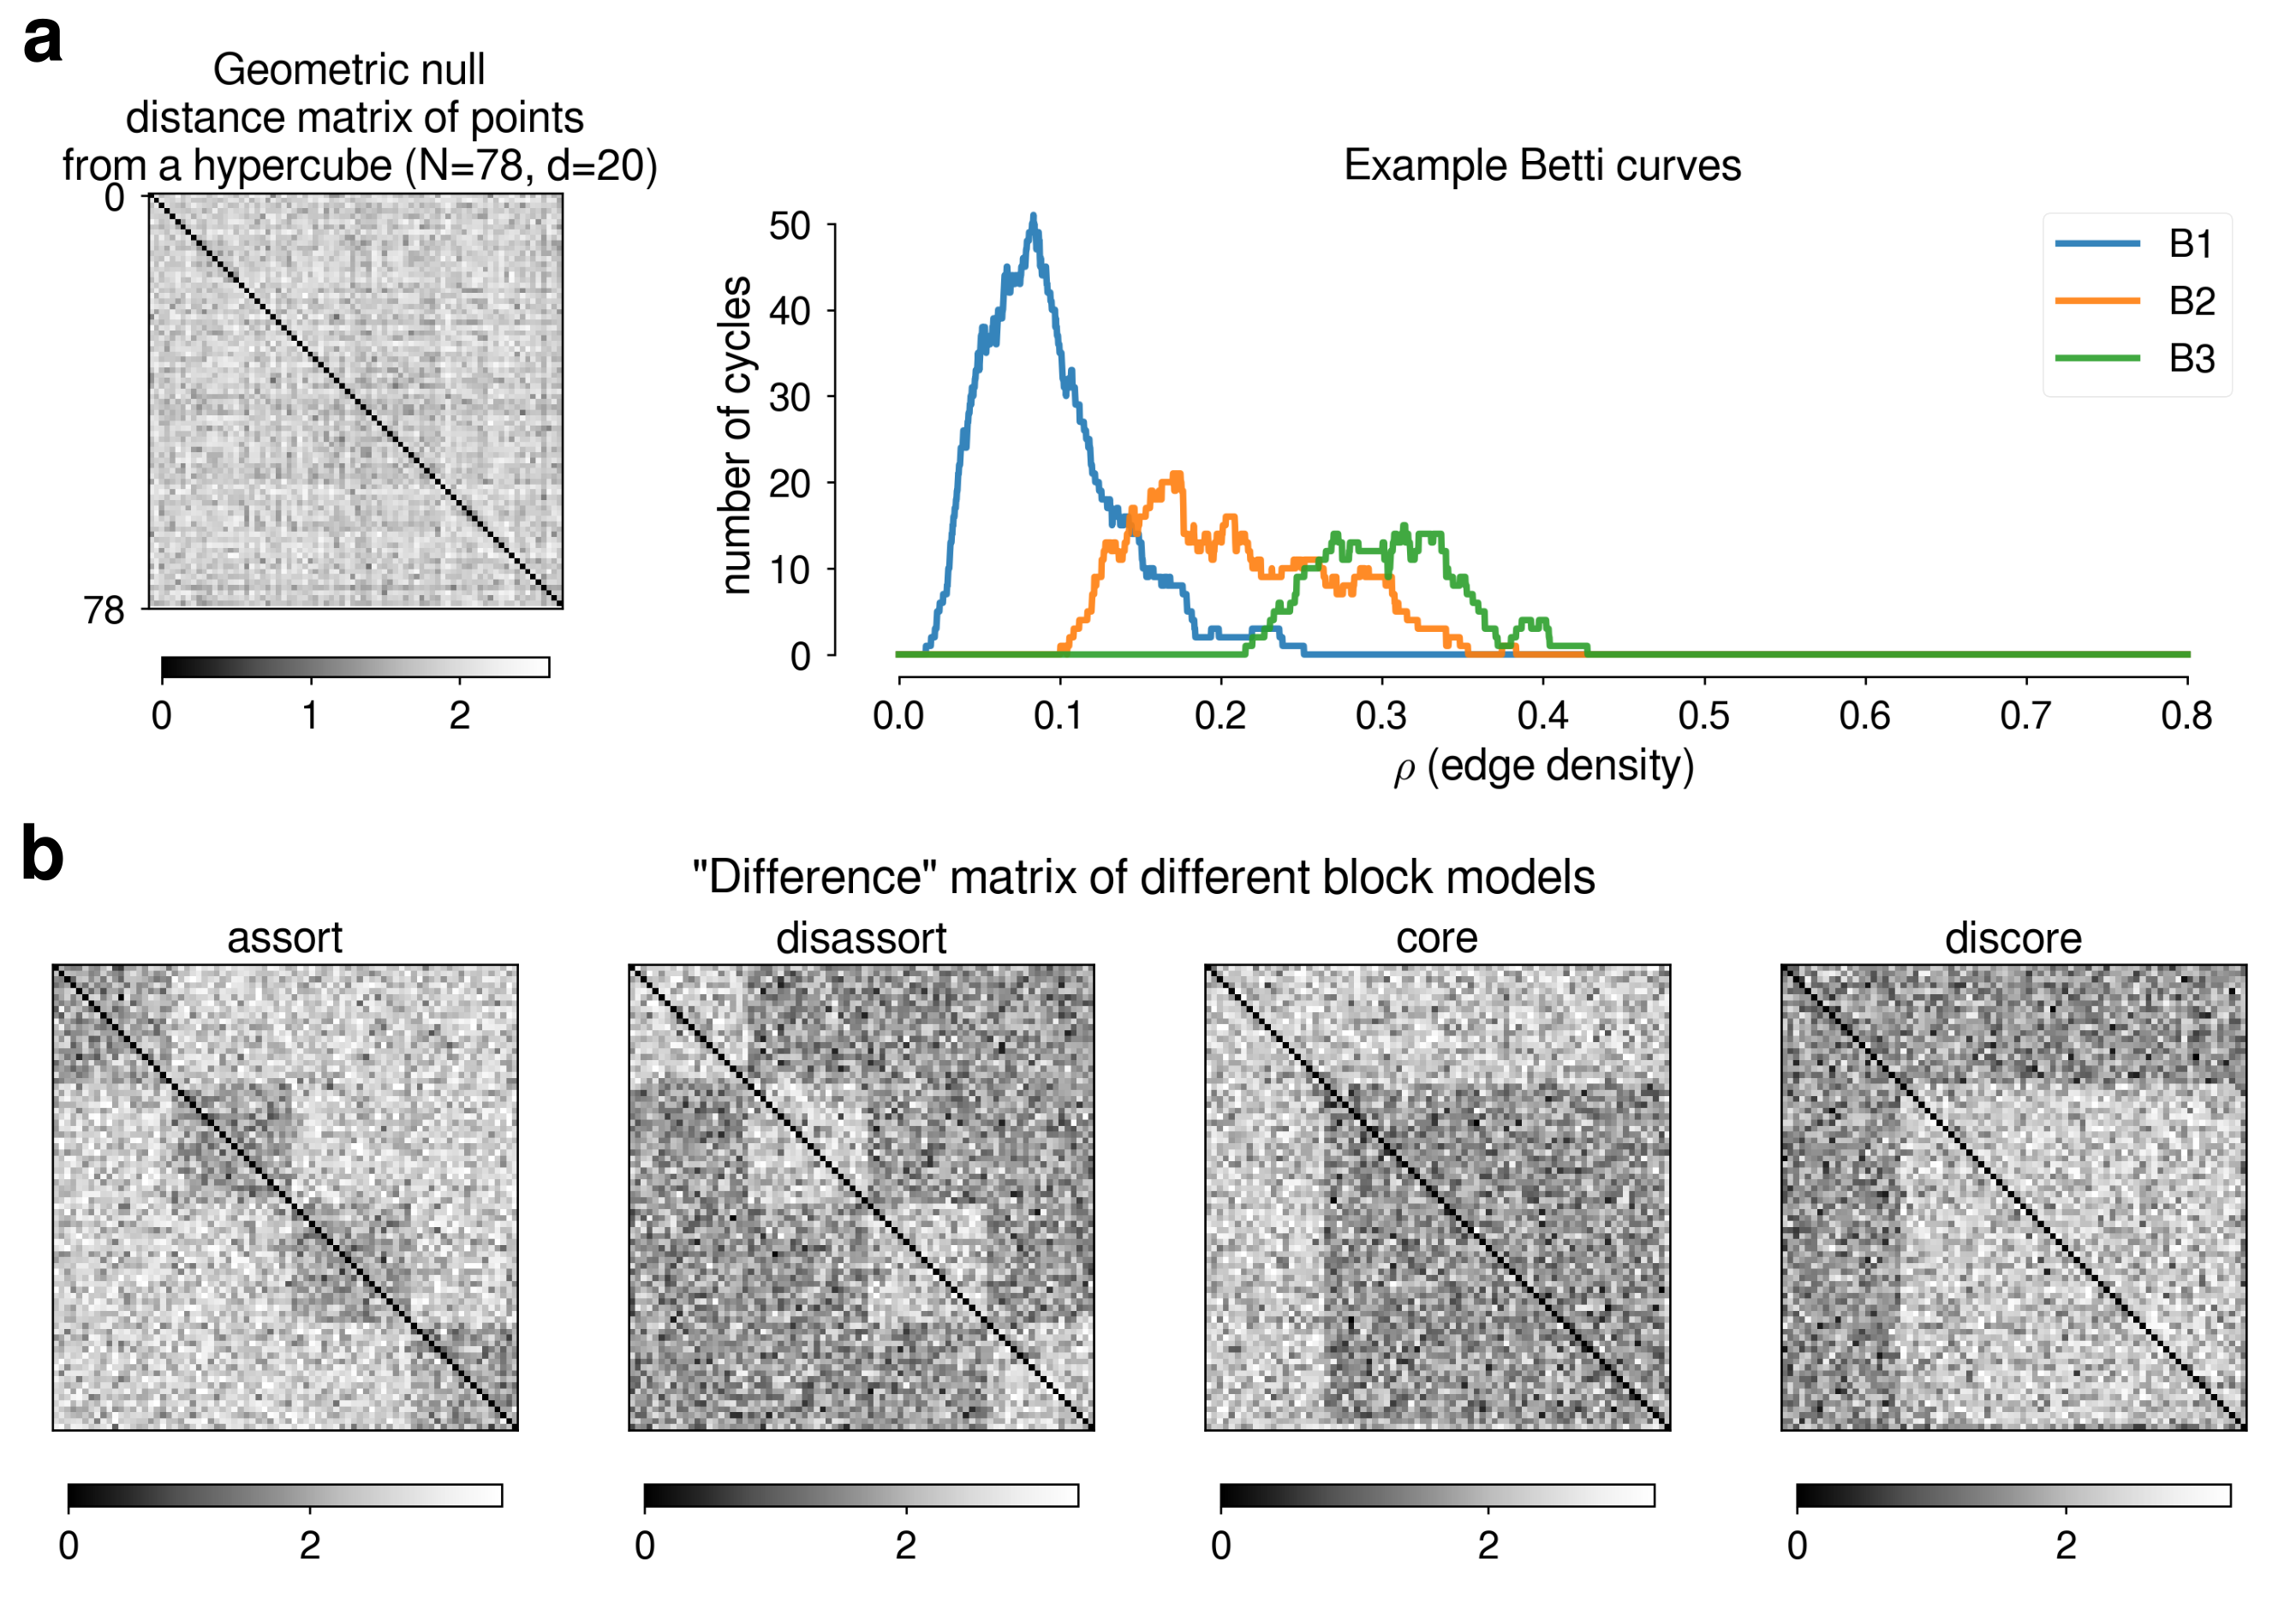
\includegraphics[width=0.55\textwidth,center]{../figures/report/Fig2.png}
    \caption{\label{fig:2}
    \textit{Null models}.
    (\textbf{a}) Example geometric null model distance matrix and the corresponding Betti curves.
    (\textbf{b}) Example ``difference'' matrices of different types of block null models
    % \vspace{-1.5em}
    }
\end{wrapfigure}\leavevmode


\subsection{Different null models}

\subsubsection*{Shuffled data}

Shuffled matrices are built by shuffling the $N(N-1)/2$ off-diagonal elements while still keeping symmetry (see \autoref{fig:1}c and \cite{Giusti2015-uo}). As stated in \cite{Giusti2015-uo}, a shuffled version is equivalent to a type of noise model where entries of the matrix are independent drawn from a uniform distribution (IID models like in \cite{Giusti2015-uo,Blevins2021-tf}). For each trial of the original data matrix, I perform 3 shuffles.

\subsubsection*{Geometric nulls}

Following \cite{Giusti2015-uo}, random geometric models are built by sampling $N=78$ points from a hypercube of dimension $d \le N$ (i.e. uniformly from $\unfdistrib{0}{1}^d$). The corresponding distance matrices (Euclidean L2 norm, see \autoref{fig:2}a) could then be used to calculate homology. For dimension $d$, I generate 30 geometric null models.

\subsubsection*{Block nulls}

Block models are constructed, taken inspiration from \cite{Blevins2021-tf}, to compare with the Purkinje population topology. Four different block configurations (30 models each) are used: \texttt{assort} (assortative), \texttt{disassort} (disassortative), \texttt{core} and \texttt{discore}. The similarity matrices $W$ are built so that the ``highly-connected" weight blocks are sampled from $\normdistrib{1.6}{0.5^2}$, and ``lowly-connected" blocks are from $\normdistrib{1}{0.5^2}$. The ``difference" matrix can be then constructed by $D = \max(W) - W$. Examples of these configurations are shown in \autoref{fig:2}.

\subsection{TDA}

\subsubsection*{Persistent homology}

Persistent homology is computed with Rips complex using difference or distance matrices. In order to compare between the data and the different null models, I perform conversion of the distance parameter to edge density $\rho$ of the graphs, and following \cite{Giusti2015-uo}, I only compare $B_1,B_2,B_3$ (to avoid confusion with entropy symbol, I use $B$ to denote homology, Betti number related analysis instead of the conventional $H$ symbol; see \autoref{fig:1}c, \autoref{fig:2}a, \autoref{fig:3}a,b). Additionally, I also analyze the ``unconverted'' version in $B_0, B_1,B_2,B_3$ (\autoref{fig:5}a). I use \href{https://gudhi.inria.fr/}{\texttt{gudhi}} for TDA.

\subsubsection*{Betti curves}

Following \cite{Giusti2015-uo,Blevins2021-tf}, I compute the Betti curve per each homology dimension per each trial or null model, which is the Betti number as a function of edge density or distance (see \autoref{fig:1}c, \autoref{fig:5}a for examples). I denote this as $\beta$ to later use for classification, with sub-sampling and smoothing.

\subsubsection*{Pairwise bottleneck distance}

For each homology dimension, the mean bottleneck distance between the data stimulus categories or null models is computed (see \autoref{fig:3}c$_1$, \autoref{fig:5}b$_1$). Taken into account these pairwise bottleneck distance matrices, I visualize the relationship between the different stimulus categories and/or null models using graphs (see \autoref{fig:3}c$_2$, \autoref{fig:5}b$_2$). For comparison with null models, I only limit visualization to geometric models of dimension $\le 10$ as all the other models are too ``far away'' from the data for any meaningful comparison.

\subsubsection*{Persistent scores and topology features}

Different features and scores are extracted from the bar codes $\{(b_i,d_i)\}$ for each homology dimension. I denote the set of these as $\phi$ to use later for classification.

\begin{itemize}
    \item \textit{Integrated Betti number}: the area under the Betti curves, using the trapezoid method
    \item \textit{Mean, median, max lifetimes}: statistics of bar code lifetimes (i.e. $|d_i - b_i|$)
    \item \textit{Persistent entropy}: entropy of the normalized lifetimes (see \cite{Myers2019-ws})
    \item \textit{Mean algebraic pq of bar codes}: $\Expected{(d_i-b_i)^p (b_i+d_i)^q}$ where $(p,q) \in \left \{(1,1),(1,2),(2,1),(1,3),(3,1) \right \}$
\end{itemize}

\subsection{MLP training for stimulus classification}

\subsubsection*{Overview}

A multi-perceptron (MLP) network with one hidden layer (50 units) is trained with inputs from activity of topology features to classify the 8 different stimulus categories. For simplicity, I consider the 8 different categories as distinct. However, future works need to consider multi-label classification instead, as the 8 different categories are combinations of 3 distinct modalities. Training is done with \texttt{pytorch} with \texttt{google-colab} resources.

\subsubsection*{Inputs}

are combinations from 3 different sources:

\begin{itemize}
    \item Average activity difference $\Delta$ between before and after stimulus onset. Specifically, denote $dF_i(a,b) = \frac{1}{b-a}\int_a^b \frac{dF_i}{F_0}(t) dt$ with $a<b$, i.e. mean activity in $t \in [a,b]$ of the i-th neuron. Then $\Delta = \{dF_i(10,12) - dF_i(5,10)\}$ where $i \in [1,N]$.
    \item Persistent scores/features $\phi$ from persistent homology analysis with actual distance (instead of edge density).
    \item Betti curves $\beta$ from persistent homology analysis with actual distance. These curves are sub-sampled and moving-average-smoothed. The Betti curves from 4 dimensions are concatenated into 1 vector to use as input.
\end{itemize}

\subsubsection*{Network}

The activation function is $\tanh$. The network is either vanilla \texttt{mlp} or with an optional batch-normalization layer after the input layer but before activation \texttt{bn}. The loss function is cross entropy loss (in the implementation, it is actually a negative log-likelihood loss with \texttt{log\_softmax} applied at the output layer)

\subsubsection*{Training}

is done in batches of size 5, for 12 epochs. Training is done either with stochastic gradient descent (SGD) with learning rate as 0.05 or Adam with learning rate as 0.001.

\subsubsection*{Classification and held-out}

The task is classification of the stimulus categories. Since there are limited trials per category, I randomly choose one trial per category as the test set while the rest are used for training. And I evaluate the mean accuracy after doing that for 100 times. The data in \autoref{table:1} are either (mean $\pm$ 95\% confidence interval = 1.96 SEM) or the maximum accuracy at the end of training across the different train-test splitting instantiations.

